%related work: kanj hat neues ergebnis mit knotenbeschränkung kleiner gleich 11...
%improved local algorithms   2012


%reactive planar spanner
%planar spanner with constant node degree
%

%pdt ist äquivalent zum pudel graph -> on the spanning ratio of pdt

%keine fehler passieren,  nachrichten sofort da sind, keine 4 punkte auf kreis, wenn ich sage dass ein punkt eine nachricht zu einem anderen sendet, ist das ein lokaler broadcast   (alle hören mit, und nur der angesprochene reagiert).

%notations und definitions  -> basics foundations
%danach related work 
\section{Related work}

In the past years several topology controls were invented and further developed.
We are interested in local algorithms only, and hence, centralized algorithms are ignored in this related work.
There are a lot of different approaches with different results.
The following is an extract of these approaches and can be divided into two main groups:
\begin{enumerate}
\item reactive algorithms
\item algorithms which produce a planar t-spanner with constant node degree
\end{enumerate}

Reactive algorithms generally need less messages as only localized algorithms due to the lack of beaconing.
They do not need the whole $k $-neighborhood of every node to function, but only a fractional amount of their direct neighbors.
As time of writing there are three reactive algorithms:
\begin{enumerate}
\item Beaconless Forwarder Planarization (BFP)
\item Guaranteed Delivery Beaconless Forwarding (GDBF) with extension
\item Reactive Partial Delaunay Triangulation (rPDT)
\end{enumerate}

\begin{table}[h!]
\centering
\begin{tabular}{ccccccc}
\hline 
Topology & reactive & planar & Eucl. stretch & Node degree & Ref. \\ 
\hline
BFP (GG) & \ding{52} & \ding{52} & $\Theta{(\sqrt{n})} $ & $\mathcal{O}(n) $ & \cite{Ruhrup2010} \\ 

GDBF & \ding{52} & \ding{52} & $\Theta{(\sqrt{n})} $ & $\mathcal{O}(n) $ & \cite{Chawla2006} \\ 

PDT & \ding{52} & \ding{52} & $7.98 $ & $\mathcal{O}(n) $ & \cite{pdt, Neumann2012} \\ 

$H_{PLOS} $ & \ding{56} & \ding{52} & $1+\epsilon $ & $\mathcal{O}(1) $ & \cite{Damian2010} \\ 

$\Updelta _{11-Spanner} $ & \ding{56} & \ding{56} & < 7 & 11 & \cite{Kanj2012} \\ 

$PuDel $ & \ding{52} & \ding{52} & $7.98 $ & $\mathcal{O}(n) $ & \cite{Xu2011} \\ 
\hline 
\end{tabular} 
\caption{Different topology controls ordered by appearance in this chapter.}
\label{table:topologies}
\end{table}

First, we describe an algorithm briefly and in the following there is a short section about properties of the produced graph.
In addition, table \ref{table:topologies} provides an overview of all discussed graphs.

The BFP-algorithm \cite{Ruhrup2010} is divided into two phases.
First, in the Selection Phase the executing node $F $ starts the algorithm by sending a RTS message. 
In the following every node, which receives this message, starts a timer corresponding to a specific delay function.
The closer a node resides to the executing node, the earlier it answers with a CTS. 
If a node $W $ overhears a CTS of a node $W' $ it checks whether or not it is contained in a certain area corresponding to node $W' $ and $F $.
This area is defined by geometric regions, in the following denoted as $Reg(A, B) $, with $A $ and $B $ being two nodes specifying this region.
The minimum region $Reg(F, W') $ is the Gabriel circle $disk(F, W') $ and the maximum region $Reg(F, W') $ is the Relative Neighborhood Graph lune over $F $ and $W' $.
The latter describes the area of the intersection of two circles around two neighboring nodes $UV $ with radii equal to $|UV| $ and with middlepoints $U $ and $V $, respectively.
Different regions cause the algorithm to use different amounts of messages.

Suppose $W $ is contained in such an area it cancels its timer and is, henceforth, called a \emph{hidden node}.
Hidden nodes further participate in the algorithm.
If a hidden node $H $ receives a message from another node $T $, it memorizes this node if $H $ lies in the former defined region. 

The Protest Phase lets hidden nodes protest against violating edges.
An edge $UV $ is called a violating edge if there is a node in $Reg(U, V) $.
If hidden nodes have nodes they memorize they restart the above timer.
As soon as a message from another hidden node $W' $ arrives at hidden node $W $, the latter checks its memorized nodes:
A node $X $ can be removed from the set of memorized nodes if $W' \in Reg(F,X) $.
If the timer of a node expires and there are still nodes which are memorized, the node sends a protest message consisting of the violating node.
The forwarder node $F $ removes violating edges when it receives protests.

This algorithm performed on each node of a graph $G $ produces a planar subgraph $G' $.
However, $G' $ is not a t-spanner of $G $ and has no constant node degree despite the underlying graphs Gabriel graph ($GG $), relative neighborhood graph ($RN $), circular neighborhood graph ($CN$) (refer to figure \ref{fig:GG_CNG_RNG} for an example of these three regions).


\begin{figure}[h!]
\centering
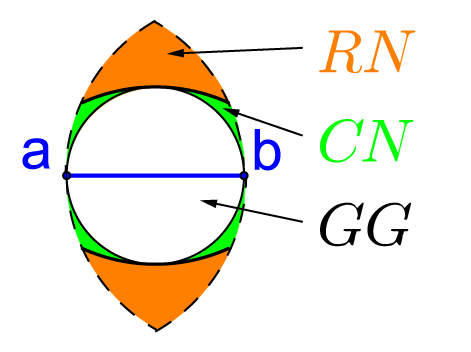
\includegraphics[width=0.4\linewidth]{eps/GG_CNG_RNG.eps}
\caption{Gabriel circle (GG), relative neighborhood (RN) and circular neighborhood (CN) between $a $ and $b $.}
\label{fig:GG_CNG_RNG}
\end{figure}

$GDBF $ is a scheme to forward messages in a network.
All messages will be greedy forwarded to the node which lies closest to the destination until a node which has no neighbors closer to the destination, called a local minimum, is reached.
From that point a recovery mode is used until the local minimum is exited and the algorithm can switch back to greedy mode.
In greedy mode the message holder broadcasts a RTS-message to all neighbors.
Every neighbor instantiates a timer with length depending on how far the neighbor is away from the destination. 
Nodes closer to the destination answer earlier.
A CTS-message is sent as soon as the timer expires and the message holder forwards the message to its sender. 
Every other node cancels its timer and remains silent.
In recovery mode a RTS message from the message holder is sent as well.
Now, all neighbors instantiate a timer corresponding to the distance to the message holder $M $ (closer nodes respond first).
If a neighbor $N $ overhears another nodes $N' $ message, it cancels its timer if $N' \in disk(M, N) $.
For more detailed information, refer to \cite{Chawla2006}.

GDBF can be extended to reactively produce a planar subgraph of a given input graph. 
Since this graph is equal to the Gabriel graph, this is not a t-spanner of the input graph and also has no constant node degree.

The understanding of the Partial Delaunay Triangulation is crucial to follow this work and, thus, it is already explained in the preamble.
PDT has a constant spanning ratio of at most $\frac{1+\sqrt{5}}{4}\pi^2 \approx 7.98 $ with respect to the Euclidean graph.
In addition, the output is a planar graph, but it has no constant bounded degree.


The second group consists of the following algorithms:
\begin{enumerate}
\item $H_{PLOS} $
\item $\Updelta _{11-Spanner} $
\item $PuDel $
\end{enumerate}

$H_{PLOS} $ (Planar Localized Optimum Spanner)\cite{Damian2010} produces a planar Euclidean spanner with stretch-factor $1+ \epsilon $ with $\epsilon >0 $ arbitrarily small and constant node degree.
However, it needs a node to be aware of its complete 2-hop-neighborhood.

$\Updelta _{11-Spanner} $ \cite{Kanj2012} constructs a spanner with an upper bound of $7 $ and a constant node degree of at most $11 $.
The obtained graph is not planar and the algorithm needs a node to know its 4-hop-neighborhood.

$PuDel $ \cite{Xu2011} is a graph which is equal to the $PDT $ graph \cite{Neumann2012} and hence, it has an Euclidean stretch-factor of $\approx 7.98 $ with respect to the Euclidean graph.
The graph is planar, it has, however, no constant node degree. 
Table \ref{table:topologies} states that $PuDel $ can be constructed reactively which is true since $PDT $ can be constructed in a reactive way and both graphs are equal.






